\documentclass{beamer}

\usepackage[utf8]{inputenc}
\usepackage[brazil]{babel}

\usepackage{verbatim}

\usepackage{graphicx}

\usepackage{listings}
\usepackage{color}

\definecolor{mygreen}{rgb}{0,0.6,0}
\definecolor{mygray}{rgb}{0.5,0.5,0.5}
\definecolor{mymauve}{rgb}{0.58,0,0.82}
\definecolor{mybckg}{rgb}{0.95,0.95,0.95}
\lstset{
  backgroundcolor=\color{mybckg},  % choose the background color; you must add \usepackage{color} or \usepackage{xcolor}
  basicstyle=\footnotesize,       % the size of the fonts that are used for the code
  breakatwhitespace=false,         % sets if automatic breaks should only happen at whitespace
  breaklines=true,                 % sets automatic line breaking
  %captionpos=b,                    % sets the caption-position to bottom
  %commentstyle=\color{mygreen},    % comment style
  deletekeywords={...},            % if you want to delete keywords from the given language
  escapeinside={\%*}{*)},          % if you want to add LaTeX within your code
  extendedchars=true,              % lets you use non-ASCII characters; for 8-bits encodings only, does not work with UTF-8
  frame=single,                    % adds a frame around the code
  keepspaces=true,                 % keeps spaces in text, useful for keeping indentation of code (possibly needs columns=flexible)
  columns=flexible,
  %keywordstyle=\color{blue},       % keyword style
  %language=bash,                   % the language of the code
  morekeywords={*,...,Hello,LS,Update},            % if you want to add more keywords to the set
  %numbers=left,                    % where to put the line-numbers; possible values are (none, left, right)
  %numbersep=5pt,                   % how far the line-numbers are from the code
  %numberstyle=\tiny\color{mygray}, % the style that is used for the line-numbers
  rulecolor=\color{black},         % if not set, the frame-color may be changed on line-breaks within not-black text (e.g. comments (green here))
  %showspaces=false,                % show spaces everywhere adding particular underscores; it overrides 'showstringspaces'
  %showstringspaces=false,          % underline spaces within strings only
  %showtabs=false,                  % show tabs within strings adding particular underscores
  %stepnumber=2,                    % the step between two line-numbers. If it's 1, each line will be numbered
  %stringstyle=\color{mymauve},     % string literal style
  tabsize=2,                       % sets default tabsize to 2 spaces
  %title=\lstname                   % show the filename of files included with \lstinputlisting; also try caption instead of title
  literate=
  {á}{{\'a}}1 {é}{{\'e}}1 {í}{{\'i}}1 {ó}{{\'o}}1 {ú}{{\'u}}1
  {Á}{{\'A}}1 {É}{{\'E}}1 {Í}{{\'I}}1 {Ó}{{\'O}}1 {Ú}{{\'U}}1
  {à}{{\`a}}1 {è}{{\'e}}1 {ì}{{\`i}}1 {ò}{{\`o}}1 {ù}{{\`u}}1
  {À}{{\`A}}1 {È}{{\'E}}1 {Ì}{{\`I}}1 {Ò}{{\`O}}1 {Ù}{{\`U}}1
  {ä}{{\"a}}1 {ë}{{\"e}}1 {ï}{{\"i}}1 {ö}{{\"o}}1 {ü}{{\"u}}1
  {Ä}{{\"A}}1 {Ë}{{\"E}}1 {Ï}{{\"I}}1 {Ö}{{\"O}}1 {Ü}{{\"U}}1
  {â}{{\^a}}1 {ê}{{\^e}}1 {î}{{\^i}}1 {ô}{{\^o}}1 {û}{{\^u}}1
  {Â}{{\^A}}1 {Ê}{{\^E}}1 {Î}{{\^I}}1 {Ô}{{\^O}}1 {Û}{{\^U}}1
  {œ}{{\oe}}1 {Œ}{{\OE}}1 {æ}{{\ae}}1 {Æ}{{\AE}}1 {ß}{{\ss}}1
  {ç}{{\c c}}1 {Ç}{{\c C}}1 {ø}{{\o}}1 {å}{{\r a}}1 {Å}{{\r A}}1
  {€}{{\EUR}}1 {£}{{\pounds}}1,
  %basicstyle=\ttfamily
}

\useoutertheme{infolines} % add a footline 
\usetheme{Frankfurt}
%\setbeamertemplate{items}[square] % changes the markers, ball: 3-dimensional balls, circle: 2-dimensional (flat) circles, rectangle: rectangles, default: triangles 
%\setbeamertemplate{section in toc}[circle]
\setbeamertemplate{section in toc}[ball unnumbered]
\setbeamertemplate{enumerate item}[square]
\setbeamertemplate{itemize item}[triangle]
\setbeamertemplate{itemize subitem}[circle]
\setbeamertemplate{blocks}[rounded][shadow=true] % add rounded corners and a shadow to the box that surrounds the theorem
\setbeamertemplate{navigation symbols}{} % disable the drawing of navigation icons

\newlength{\wideitemsep}
\setlength{\wideitemsep}{\itemsep}
\addtolength{\wideitemsep}{10pt}
\let\olditem\item
\renewcommand{\item}{\setlength{\itemsep}{\wideitemsep}\olditem}

\title[Localização para Robôs Móveis]{Localização \textit{indoor} para robôs móveis}
\author[Edileuton H. de Oliveira]{Edileuton Henrique de Oliveira}
\institute[UFPR]{
  Departamento de Informática\\
  Universidade Federal do Paraná\\
  Bacharelado em Ciência da Computação\\
  Trabalho de Graduação\\
  Orientador: Prof. Eduardo Todt.
}

\usepackage{remreset}
\makeatletter
\@removefromreset{subsection}{section}
\makeatother


\begin{document}
%\maketitle

\begin{comment}
\frame{\titlepage}

\frame{
\frametitle{Sumário}
\tableofcontents
}
\end{comment}

\begin{frame}
  \titlepage
\end{frame}

\section*{Sumário}
\begin{frame}
\tableofcontents
\end{frame}

\setcounter{subsection}{1}

%\section{Introduçao}

\section{Robôs Móveis}

\begin{frame}{Robôs Móveis}
\begin{itemize}
 \item São sistemas incorporados no mundo real que se movem autonomamente e interagem com ele para realizar suas tarefas.
 \item Aplicações: limpeza, corte de grama, detectar riscos, explorações de ambientes desconhecidos, 
vigilância autônoma, resgatar sobreviventes e assistência a idosos ou pessoas com alguma incapacidade.
  \item Principais tarefas: planejamento de caminho, navegação,  
evitar obstáculos, controle de motores, \textbf{localização}, \textbf{construção e atualização de mapas}.

\end{itemize}
\end{frame}

\begin{frame}{Construção de Mapas}
A tarefa de mapeamento corresponde à atribuição de valores aos elementos do mapa, relacionando cada um a uma certa 
posição nele.
\begin{itemize}
 \item \textbf{Mapas Métricos}
    \begin{itemize}
    \item Mapa detalhado do ambiente, dividido em uma rede de células.
    \item Cada célula contem informações do ambiente como espaço ocupado por um objeto, 
    espaço livre para navegação, etc.
    \item Localização é mais precisa e menos sujeita a ambiguidades.
    \end{itemize}

 \item \textbf{Mapas Topológicos}
      \begin{itemize}
    \item  Marcos e relações são os elementos dos mapas topológicos, concentra-se apenas em pontos de interesse.
    \item Essas relações podem ser de vários tipos, tais como o deslocamento
relativo entre dois marcos, a existência de um caminho entre eles,
quantidade de energia gasta em um caminho entre marcos, etc.
    \end{itemize}
\end{itemize}
\end{frame}

\begin{frame}{Localização}

 \begin{itemize}
  \item A obtenção da posição e orientação do robô no mapa: \textbf{pose($x$, $y$, $\theta$)}.
  
  \item Identificação e subsequente triangulação por ângulos e por distância dos \textit{landmarks}.
  
  \item A identificação dos \textit{landmarks} 
 é feita fazendo observações do ambiente utilizando seus sensores(sonar, laser, câmera).
 
  \item O robô deve ser capaz de lidar com os erros de medição dos sensores, 
 incertezas e informações incompletas.
\end{itemize}
\end{frame}

\begin{frame}{Localização Probabilística}
\begin{itemize}
  \item Ao invés de calcular a posição exata, calcula-se a 
  probabilidade do robô estar numa certa posição.
  \item A localização probabilística nos da a distribuição de probabilidade de todas as possíveis 
 configurações do robô: \textit{\textbf{belief}}.
  \item Principais abordagens: \textbf{localização de Markov} e \textbf{filtro de Kalman}.
  \item \textbf{SLAM}
\end{itemize}
\end{frame}
 \begin{comment}
\begin{frame}{Modelo de Movimento e Percepção}
\begin{itemize}
\item Quando o robô se movimenta a incerteza de sua posição aumenta. 
\item A cada deslocamento do robô faz a atualização da distribuição de probabilidade que pode ser dividida em 2 passos:
   \begin{itemize}
  \item \textbf{Atualização de ação}: o robô se move e estima sua posição através estimação da odometria: incerteza aumenta.
  \item \textbf{Atualização de percepção}: o robô faz uma observação usando seus sensores e corrige sua posição, 
  combinando seu \textit{belief} com a probabilidade das observações feitas: incerteza diminui.
 \end{itemize}
 
 \item Desse modo, a cada movimento o robô pode obter uma melhor estimativa de sua real posição.
 \end{itemize}
\end{frame}
 

\begin{frame}{Localização de Markov}
\begin{itemize}
 \item Encontra caminhos mínimos de maneira rápida e sem ciclos % pois utiliza o Dijkstra
 \item Utiliza menos largura de banda % pois nao envia a tabela de roteamento inteira, envia somente o estado de seus enlaces 
 \item É possível utilizar diversas métricas no calculo do caminho mínimo % menor custo, maior vazão, maior confiabilidade
 \item Mantém mais de um caminho mínimo para um dado destino % caminhos devem possuir valores de métrica idênticos  % aumenta eficiencia pois possibilita a divisão do trafego 
\end{itemize}
\end{frame}

\begin{frame}{Localização filtro de Kalman}
\begin{itemize}
 \item Encontra caminhos mínimos de maneira rápida e sem ciclos % pois utiliza o Dijkstra
 \item Utiliza menos largura de banda % pois nao envia a tabela de roteamento inteira, envia somente o estado de seus enlaces 
 \item É possível utilizar diversas métricas no calculo do caminho mínimo % menor custo, maior vazão, maior confiabilidade
 \item Mantém mais de um caminho mínimo para um dado destino % caminhos devem possuir valores de métrica idênticos  % aumenta eficiencia pois possibilita a divisão do trafego 
\end{itemize}
\end{frame}
\end{comment}

\begin{comment}
\begin{frame}{Mapas Métricos}
Periodicamente, cada roteador:
\begin{itemize}
 \olditem verifica o estado de seus enlaces % através do envio de pequenas mensagens
 \olditem envia as informações do estado dos enlaces aos roteadores adjacentes % quando ocorre mudanças na rede, stop() quando a ocorre mais troca de mensagem
\end{itemize}
\end{frame}

\begin{frame}{Mapas Topológicos}
Periodicamente, cada roteador:
\begin{itemize}
 \olditem verifica o estado de seus enlaces % através do envio de pequenas mensagens
 \olditem envia as informações do estado dos enlaces aos roteadores adjacentes % quando ocorre mudanças na rede, stop() quando a ocorre mais troca de mensagem
\end{itemize}
\end{frame}


\begin{frame}{SLAM}
\begin{itemize}
  \item O robô inicia a navegação em uma localização desconhecida e em um ambiente desconhecido.
  \item Constrói um mapa desse ambiente de maneira incremental.
  \item Utiliza esse mapa simultaneamente para calcular a sua localização.
  \item Principais abordagens:
  \begin{itemize}
  \item \textbf{Extended Kalman Filter SLAM}. 
  \item \textbf{Filtro de partículas}.
  \item \textbf{GraphSLAM}.
  \end{itemize}
\end{itemize}
\end{frame}
\end{comment}
\section{Localização baseada em Wireless sensor networks - WSNs}

\begin{frame}{Localização baseada em \textit{Wireless sensor networks} - WSNs}
\begin{itemize}
 \item Coleta informações em um campo monitorado.
 \item Nodos da rede podem ser estáticos ou móveis.
 \item Geralmente requerem que os nodos conhecidos, estejam dentro 
	do raio de comunicação dos sensores em comum.
  \item A posição de um certo nodo pode ser obtida 
  a partir da posição ou direção dos nodos conhecidos por ele.
\end{itemize}
\end{frame}

\begin{frame}{Principais abordagens utilizando WSNs}
\begin{itemize}
  \item Principais abordagens:
    \begin{itemize}
     \item \textbf{TOA}(\textit{Time of Arrival}).
     \item \textbf{TDOA}(\textit{Time Difference of Arrival}).
     \item \textbf{AOA}(\textit{Angle of Arrival}).
     \item \textbf{RSS}(\textit{Received Signal Strength}).
    \end{itemize}

 \item Sofrem interferência de obstáculos como paredes, 
   móveis e outros objetos, trafego de pessoas, além de outros fatores como temperatura ambiente, 
   umidade do ar, outros sinais, etc.
\end{itemize}
\end{frame}

\begin{comment}
\begin{frame}{TOA(\textit{Time of Arrival})}

\begin{itemize}
 \item Tempo medido em que um sinal chega a um
receptor pela primeira vez depois de emitido.
\item O valor medido é o tempo de transmissão somado ao
atraso do tempo de propagação.
\item Este atraso,$t_{i,j}$, entre a transmissão do sensor i e recepção do sensor j, é igual a distância entre o transmissor e o receptor, 
$d_{i,j}$, dividido pela velocidade de propagação do sinal, $v_{p}$.

\end{itemize}
\end{frame}

\begin{frame}{TDOA(\textit{Time Difference of Arrival})}
\begin{itemize}
 \item Os algoritmos de TDOA fazem a medição da diferença no tempo de recepção
de sinais de diferentes estações de base.
  \item Supondo que o nodo está na linha de visão de dois BSs,
  o nodo deve situar-se em uma hipérbole. 
  \item Uma segunda hipérbole, pode ser obtido através de uma medição adicional de TDOA envolvendo
um terceiro BS. 
  \item A posição do nodo pode ser identificada como o ponto de intersecção
das duas hipérboles.
\end{itemize}
\end{frame}


\begin{frame}{AOA(\textit{Angle of Arrival})}
\begin{itemize}
 \item A Localização baseada em AOA envolve a medição do ângulo de chegada de um sinal de uma BS
a um receptor ou vice-versa. 
 \item Uma única medida produz uma linha reta 
entre a \textit{base station} e o receptor. 
  \item A medida do ângulo de chegada com outra \textit{base station}
produzirá uma segunda linha reta e a intersecção das duas linhas, vai fornecer a posição
do dispositivo.
\end{itemize}
\end{frame}
\end{comment}
\begin{frame}{RSS(\textit{Received Signal Strength})}
Há três métodos de localização que utilizam a medição de RSS:
\begin{itemize}
 \olditem \textbf{Estação base mais forte}.
 \begin{itemize}
  \item A localização de um nodo da rede pode ser estimado como a posição do \textit{Access Points}(AP) mais próximo, no 
	qual o nodo se comunicou.
 \end{itemize}

 \olditem \textbf{Modelo de propagação}.
  \begin{itemize}
  \item A medição do sinal no receptor e o valor obtido indica a distância até o transmissor.
  \item A localização é obtida fazendo triangulação com outros 3 APs, cuja posição conhecida.
 \end{itemize}
 \olditem \textbf{\textit{Fingerprinting}}, composta por duas fases:
  \begin{itemize}
  \item Aprendizado: constrói uma tabela para cada coordenada de amostras.
  \item Determinação: o nodo informa uma amostra do RSS, o registro que mais se aproxima da amostra informada é adotada como atual posição do nodo.
 \end{itemize}
\end{itemize}
\end{frame}


\section{Android} % Detalhe os experimentos que vc fez no NS-3
\begin{frame}{Android}
\begin{itemize}
\item O Android é um sistema operacional baseado no núcleo do Linux para dispositivos móveis, 
desenvolvido pela \textit{Open Handset Alliance}.

 \item Apresenta vários recursos que podem facilmente empregados na robótica como
câmeras, GPS, aceleradores gráficos 2D e 3D, \textit{bluetooth} e wifi.

\item Suporta diversos sensores como barômetro, magnetômetro, acelerômetro, 
 sensor de proximidade, sensor de pressão, termômetro e compasso. 
 
 \item Possui um rico ambiente de desenvolvimento provido pelo Android SDK com documentação farta.

\end{itemize}
\end{frame}

\begin{frame}{Arquitetura do Sistema Operaciona Android}
\begin{figure}[hb]
\centering
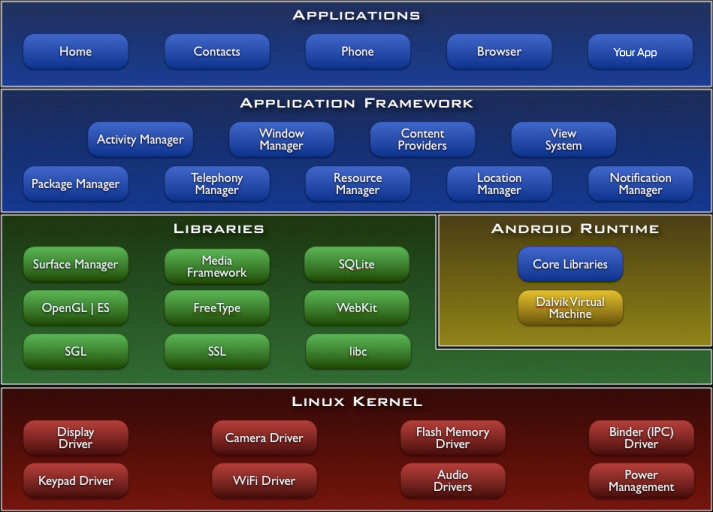
\includegraphics[scale=0.38]{../images/Android-architecture.jpg}
\caption{Arquitetura Android\cite{android1}. }
\label{fig:android-arc}
\end{figure}
\end{frame}

\begin{frame}{Componentes de uma Aplicação Android}
\begin{itemize}
 \item Activity.
 \item Services.
 \item Broadcast Receiver.
 \item Content Providers.
\end{itemize}
\end{frame}

\section{Implementação}
\begin{frame}{Técnica implementada}
\begin{itemize}
 \item Implementa o RSS \textit{fingerprinting}.
 \item O algoritmo utiliza o preceito da correlação espacial das localidades adjacentes.
 \item Obtém-se um conjunto de pontos que definem uma região de onde o aparelho possa estar.
 \item A posição final do aparelho 
  e obtida através do centroide desse conjunto de pontos.
\end{itemize}
\end{frame}

\begin{frame}{Aprendizado e Determinação}
\begin{itemize}
 \olditem \textbf{Aprendizado:}
  \begin{enumerate}
    \item Constrói um mapa de \textit{fingerprints}.
    \item O \textit{fingerprint} é composto da média de 8 amostras do RSS de cada AP.
  \end{enumerate}
 
 \olditem \textbf{Determinação:}
    \begin{enumerate}

    \item Obtêm-se o \textit{fingerprint} da localidade do aparelho.
    \item Para cada conjunto de três APs do \textit{fingerprint} obtém-se um ponto, onde 
    esse ponto é resultado da busca pela menor distância euclidiana entre os dados informados e os dados
    previamente coletados.
    \item Assim obtêm-se um conjunto de $n$ pontos.
    \item Calcula-se o centroide desses pontos: $c(x_c,y_c) = (\frac{1}{n}\sum_{i=1}^{n}x_{i},\frac{1}{n}\sum_{i=1}^{n}y_{i})$.  
    \end{enumerate}
\end{itemize}
\end{frame}

\begin{frame}{Tecnologias utilizadas}
\begin{itemize}
 \item Android SDK.
 \item Escrito em Java e XML.
 \item LG Nexus 4 com Android KitKat 4.4.4.
\end{itemize}
\end{frame}

\begin{frame}{Esquema da implementação}
  \begin{figure}[hbt]
  \centering
  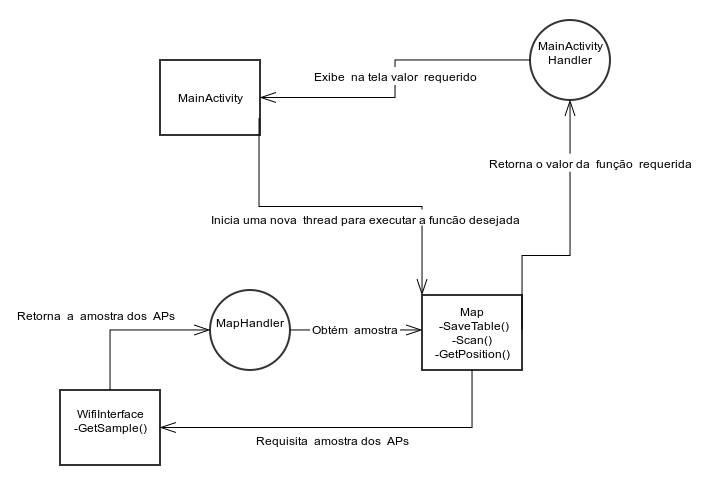
\includegraphics[scale=0.39]{../images/apptg.png}
  \caption{Esquema de interação entra as classes}
  \label{fig:appSchema}
  \end{figure}
\end{frame}

\begin{frame}{Testes}
Foram coletados \textit{fingerprints} de 67 locais distintos,
  onde o incremento de um no eixo $x$ ou $y$ significa um metro do primeiro andar do DINF.
   
   \begin{figure}[hbt]
  \centering
  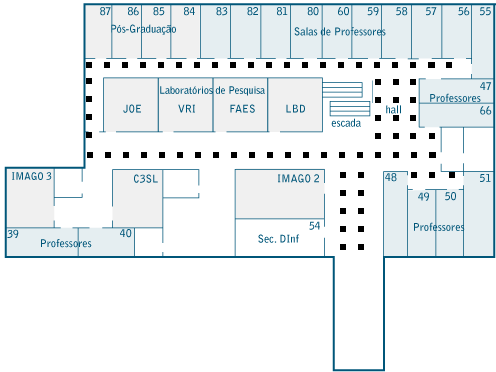
\includegraphics[scale=0.4]{../images/TTmapadinf_andar1_492x327.png}
  \caption{Mapa do primeiro andar do Departamento de Informática da UFPR.}
  \label{fig:mapaDinf}
  \end{figure}
\end{frame}

\begin{frame}{Resultados}
 Foram realizados 35 testes, onde:
  \begin{itemize}
      \item 22,8\% das estimativas possuem precisão de 1 metro ou menos.
      \item 77,1\% das estimativas possuem precisão de 3 metros ou menos.
      \item 91,4 \% das estimativas possuem precisão de 5 metros ou menos.
     \end{itemize}
\end{frame}

\section{Conclusão}
\begin{frame}{Conclusão}
\begin{itemize}
 \item Precisão satisfatória, considerando um raio de 2 até 5 metros da posição real do aparelho.
 \item A oscilação do RSS e a semelhança dos \textit{fingerprints} em um raio de até 5 metros do aparelho
  dificultaram uma precisão mais aguda.
  \item O ambiente deve ser lavado em consideração, já que o ambiente escolhido é bastante favorável a abordagem escolhida, dado
      o grande número de APs presentes.
 \item Essa técnica pode ser bastante proveitosa na localização de robôs móveis, pois há 
      a possibilidade de adicionar mais características para distinguir os \textit{fingerprints} com 
      dados coletados por outros sensores do robô(câmera, laser, sonar).
\end{itemize}
\end{frame}

\end{document}
